\documentclass{beamer}
\usepackage{listings}
\lstset{
%language=C,
frame=single, 
breaklines=true,
columns=fullflexible
}
\usepackage{subcaption}
\usepackage{url}
\usepackage{tikz}
\usepackage{tkz-euclide} % loads  TikZ and tkz-base
%\usetkzobj{all}
\usetikzlibrary{calc,math}
\usepackage{float}
\newcommand\norm[1]{\left\lVert#1\right\rVert}
\renewcommand{\vec}[1]{\mathbf{#1}}
\usepackage[export]{adjustbox}
\usepackage[utf8]{inputenc}
\usepackage{amsmath}
\usetheme{Boadilla}

\title{My Presentation}
\author{Siddhartha Pothukuchi}
\institute{Indian Institute of Technology, Bhilai.}
\date{\today}
\begin{document}


\begin{frame}
\titlepage
\end{frame}
\section{Question}
\begin{frame}
\frametitle{Question}
\begin{block}{Exercise 8.1(Q no.28)}
In right triangle ABC, right angled at C, M is
the mid-point of hypotenuse AB. C is joined to
M and produced to a point D such that DM =
CM. Point D is joined to point B. Show that:
\newline
\hyperlink{a}{\beamerbutton{a)$\triangle  AMC  \cong   \triangle  BMD $}}
\newline
\hyperlink{b}{\beamerbutton{b)$\triangle DBC $ is a right angle.}}
\newline
\hyperlink{c}{\beamerbutton{c)$\triangle  DBC  \cong  \triangle  ABC $}}
\newline
\hyperlink{d}{\beamerbutton{d)CM = $\frac{1}{2}$ AB}}

\end{block}
\end{frame}

\section{\textbf{Construction}}
\subsection*{Codesandfigures}
\begin{frame}[fragile]
\frametitle{Codes and Figures}
\tiny
\begin{flushleft}
The python code for the figure is
\begin{lstlisting}
./code/traingle.py
\end{lstlisting}
The latex- tikz code is
\begin{lstlisting}
./figs/triangle.tex
\end{lstlisting}
The above latex code can be compiled as standalone document
\begin{lstlisting} 
./figs/triangle_fig.tex
\end{lstlisting}
\end{flushleft}.
%\begin{columns}
%\column{0.5\textwidth}
\begin{figure}
\begin{flushleft}
\begin{subfigure}{0.2\textwidth}
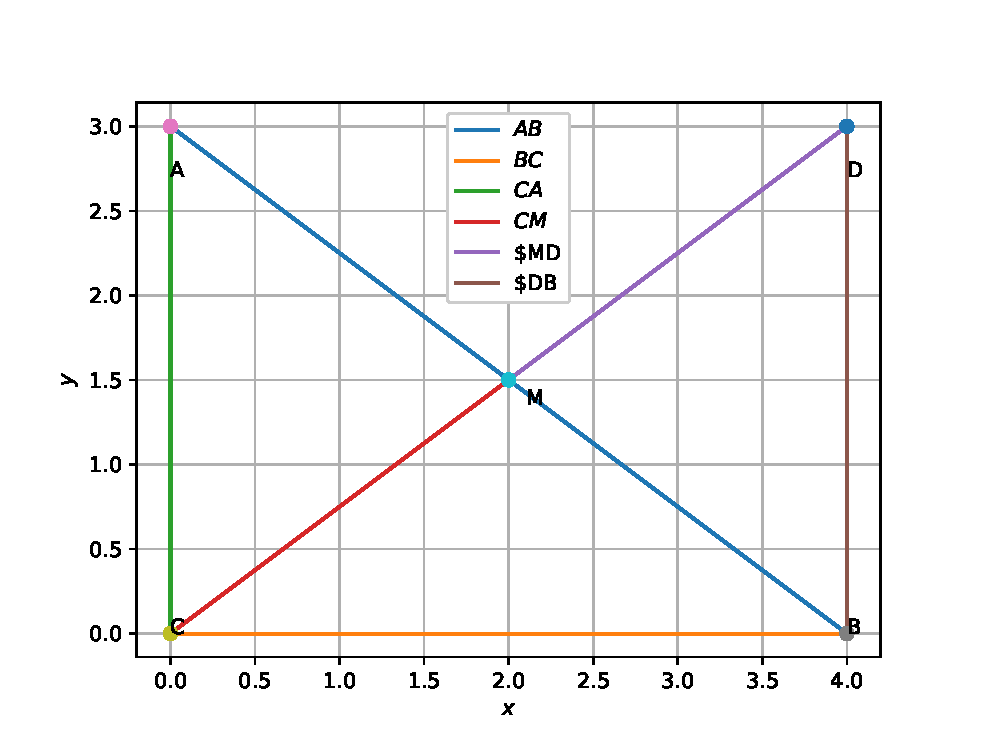
\includegraphics[scale=0.275]{./figs/triangle.eps}
\caption{\tiny By Python}
\end{subfigure}
%
\begin{subfigure}{0.65\textwidth}
\begin{flushright}


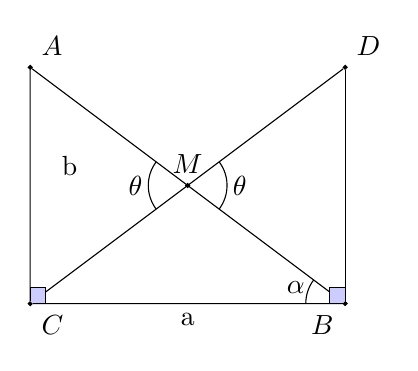
\begin{tikzpicture}
[scale=1,>=stealth,point/.style={draw,circle,fill = black,inner sep=0.5pt},]

%Triangle sides
\def\a{4}
\def\b{3}
\def\c{sqrt(\a^2+\c^2)}



%Labeling points
\node (A) at (0,\b)[point,label=above right:$A$] {};
\node (B) at (\a, 0)[point,label=below left:$B$] {};
\node (C) at (0, 0)[point,label=below right:$C$] {};
\node (M) at (\a*0.5,\b*0.5)[point,label=above:$M$] {};
\node (D) at (\a,\b)[point,label=above right:$D$] {};


%Drawing triangle ABC
\draw (A) -- node[left] {$\textrm{}$} (B) -- node[below] {$\textrm{a}$} (C) -- node[above,xshift=5mm] {$\textrm{b}$} (A);

%Joining CD
\draw (C)--(D);
%Joining BD
\draw (B)--(D);

%Drawing and marking angles
\tkzMarkAngle[fill=orange!40,size=0.5cm,mark=](A,M,C)
\tkzMarkAngle[fill=orange!40,size=0.5cm,mark=](B,M,D)
\tkzMarkAngle[fill=green!40,size=0.5cm,mark=](A,B,C)
\tkzMarkRightAngle[fill=blue!20,size=.2](A,C,B)
\tkzMarkRightAngle[fill=blue!20,size=.2](D,B,C)
\tkzLabelAngle[pos=0.65](A,M,C){$\theta$}
\tkzLabelAngle[pos=0.65](B,M,D){$\theta$}
\tkzLabelAngle[pos=0.65](A,B,C){$\alpha$}


\end{tikzpicture}

\caption{\tiny By Latex-tikz}
\end{flushright}
\end{subfigure}
\end{flushleft}
%
\end{figure}
\end{frame}
\subsection*{Construction methods}
\begin{frame}[fragile]
\footnotesize
\frametitle{Construction method}
\begin{columns}
\begin{column}{0.5\textwidth}
The tables below are the values used for constructing the triangles in both Python and Latex-Tikz.
\begin{table}[htbp]
\centering
  \resizebox{0.5\textwidth}{!}{\begin{minipage}{\textwidth}
\begin{tabular}{ |p{3cm}|p{3cm}|  }
\hline
 \multicolumn{2}{|c|}{Initial Input Values.} \\
\hline
a & 4\\
\hline
b & 3\\
\hline
$\angle(ACB)$ & $90^{\circ}$ \\
\hline
\end{tabular}
\end{minipage}}
\caption{\tiny To construct $\triangle ACB$}
\end{table}
The steps for constructing $\triangle ACB$ are
\newline
$$(i)\vec{C}= \begin{pmatrix}0\\0\end{pmatrix}
(ii)\vec{A}=\begin{pmatrix}0\\3\end{pmatrix}
(iii)\vec{B}=\begin{pmatrix}4\\0\end{pmatrix}$$
\end{column}
\begin{column}{0.5\textwidth}
Since, $\vec{M}$ is the midpoint of $\vec{AB}$ and $\vec{CD}$
\\
$$\vec{M}=(1/2)(\vec{A}+\vec{B})
\vec{M}=\begin{pmatrix}2\\1.5\end{pmatrix}$$,
\\
$$\vec{D}=2\vec{M}
\vec{D}=\begin{pmatrix}4\\3\end{pmatrix}$$
\begin{table}[H]
\centering
\resizebox{0.5\textwidth}{!}{\begin{minipage}{\textwidth}
\begin{tabular}{ |p{3cm}|p{3cm}|  }
\hline
 \multicolumn{2}{|c|}{Derived Values for $triangle DCB$.} \\
\hline
$\vec{M}$ & $$\begin{pmatrix}2\\1.5\end{pmatrix}$$\\				
\hline
$\vec{D}$ & $$\begin{pmatrix}4\\3\end{pmatrix} $$\\
\hline
\end{tabular}
\end{minipage}}
\caption{\tiny To construct $\triangle DCB$}
\end{table}
\end{column}
\end{columns}
\end{frame}
\section*{\textbf{Solution}}
\begin{frame}[fragile]
\footnotesize
\frametitle{Solution}
\begin{columns}
\begin{column}{0.5\textwidth}
From the figure, lets assume $\vec{C}$ to be the origin.
\newline
\begin{figure}[H]
\input{./figs/triangleABC.tex}
\caption{$\triangle ACB$}
\end{figure}
$\vec{C}=0, 
\norm{\vec{CA}}=b 
\norm{\vec{CB}}=a$
\newline
$\vec{M}$ is the position vector of mid-point of $\vec{BA}$.
\newline
$\vec{CM} = \vec{CB}+\vec{BM}$ [$\vec{BM}=(1/2)*\vec{BA}$]
\newline
$$\vec{CM} =\begin{pmatrix}a\\0\end{pmatrix}+\begin{pmatrix}-a\\b/2\end{pmatrix}$$
\end{column}
\begin{column}{0.5\textwidth}
Therefore, $$\vec{CM}=\begin{pmatrix}a/2\\b/2\end{pmatrix}$$
\begin{figure}[H]
\input{./figs/triangleDBC.tex}
\caption{$\triangle DBC$}
\end{figure}
From the figure, $\vec{CD}=2(\vec{CM})$
\newline
$$\vec{CD}=\begin{pmatrix}a\\b\end{pmatrix}$$
\end{column}
\end{columns}
\end{frame}
\subsection{a}
\begin{frame}
\frametitle{Solution a)}
\footnotesize
\label{a}

$\triangle AMC$ and $\triangle DMB$ are congruent to each other by SAS congruency.
\newline
(i) Side AM  is equal to the corresponding side BM  [As M is midpoint of AB]
\newline
(ii)Side CM of is equal to corresponding side DM [As M is midpoint of DC]
\newline
(iii)$\angle AMC$ = $\angle DMB$ [ Vertically Opposite Angles]
\\
Hence, proved
\end{frame}
\subsection{b}
\begin{frame}
\frametitle{Solution b)}
\footnotesize
\label{b}
In $\triangle ACB$  $(\norm{\vec{BA}})^2= a^2+b^2$
Since $\angle ACB$ = 90$^{\circ}$[ Pythagorus theorem]
\newline
In $\triangle DBC$ 
$cos \angle DBC= [((a^2+b^2-(\norm{\vec{CD}})^2)/2ab)] $
With the given vector values we get norm of $(\norm{\vec{BA}})=(\norm{\vec{CD}})$
\newline
$cos\angle DBC =[((a^2+b^2-(\norm{\vec{CD}})^2)/2ab)]$
$cos\angle DBC$=0
\newline
Therefore, $\angle DBC$ is right angle
\end{frame}
\subsection{c}
\begin{frame}
\frametitle{Solution c)}
\footnotesize
\label{c}
$\triangle ACB$ and $\triangle DCB$ are congruent to each other in SAS congruency.
\\
(i)Both the triangles have a common base , a.
\newline
(ii)AC = DB by using distance formula
\newline
(iii)$\angle ACB$ = $\angle DBC$ = 90$^{\circ}$ [ From Solution b)]
\\
Hence, proved.

\end{frame}
\subsection{d}
\begin{frame}
\frametitle{Solution d)}
\footnotesize
\label{d}
Since $\vec{CM}$ is halfway of $\vec{CD}$
\newline
$\norm{\vec{CM}}=\norm{\vec{CD}}$
\newline
From Solution b) it is clear that $\norm{\vec{CD}}=\norm{\vec{BA}}$
\newline
Therefore $\norm{\vec{CM}}=\frac{1}{2}\norm{\vec{AB}}$
\\
Hence, proved.
\end{frame}







\end{document}
